\chapter{Approximation Algorithms}
An algorithm for an optimization problem that yields a ``nearly''
optimal solution is called an approximation algorithm.
$0<C_{n}*$ cost of an optimal solution for an input of size
$n$ (e.g. length of a shortest path). $0<C_{n}$ cost of a solution
produced by an approximation algorithm. If 
$max(\frac{C_{n}}{C_{n}*},\frac{C_{n}*}{C_{n}})=\rho (n)$ then
the algorithm has an approximation ratio of $\rho (n)$.\\
(Remark: $\rho (n) \ge 1$)\\
$\rho (n) = 1$: optimal, $\rho(n) >> 1$: bad approximation\\
Trade-off: Cost of the approximation algorithm vs. quality of approximation.\\
An approximation scheme for an approximation problem is an 
algorithm with 2 inputs: $Problem + \epsilon>0$ such that
the algorithm is a $(1 + \epsilon)$ - approximation algorithm.\\
The approximation scheme is a polynomial time approximation
scheme if for each $\epsilon > 0$ the induced algorithm runs in polynomial time in $n$.
It is fully polynomial if it is polynomial in $n$ and in $1/\epsilon$.
\begin{example}
$O(n^(\frac{2}{3}))$, if $\epsilon' = \frac{3}{4}$ $O(n^(\frac{8}{\epsilon}))$ cost, i.e.
the costs are rising but not by a constant factor.
\end{example}
\begin{example}
$O((1/\epsilon)^2 * n^3)$ fully polynomial. $\epsilon = \frac{\epsilon}{4}
O(16*(\frac{1}{\epsilon}^2 * n^3))$.
\end{example}
\section{Heuristic Approaches}
\emph{Vertex Cover}: Given an undirected graph $G=(V,E)$ without parallel edges and without loops,
we look for a minimal set $V'$ of nodes such that each edge has at least one endpoint in $V'$.
\begin{example*}
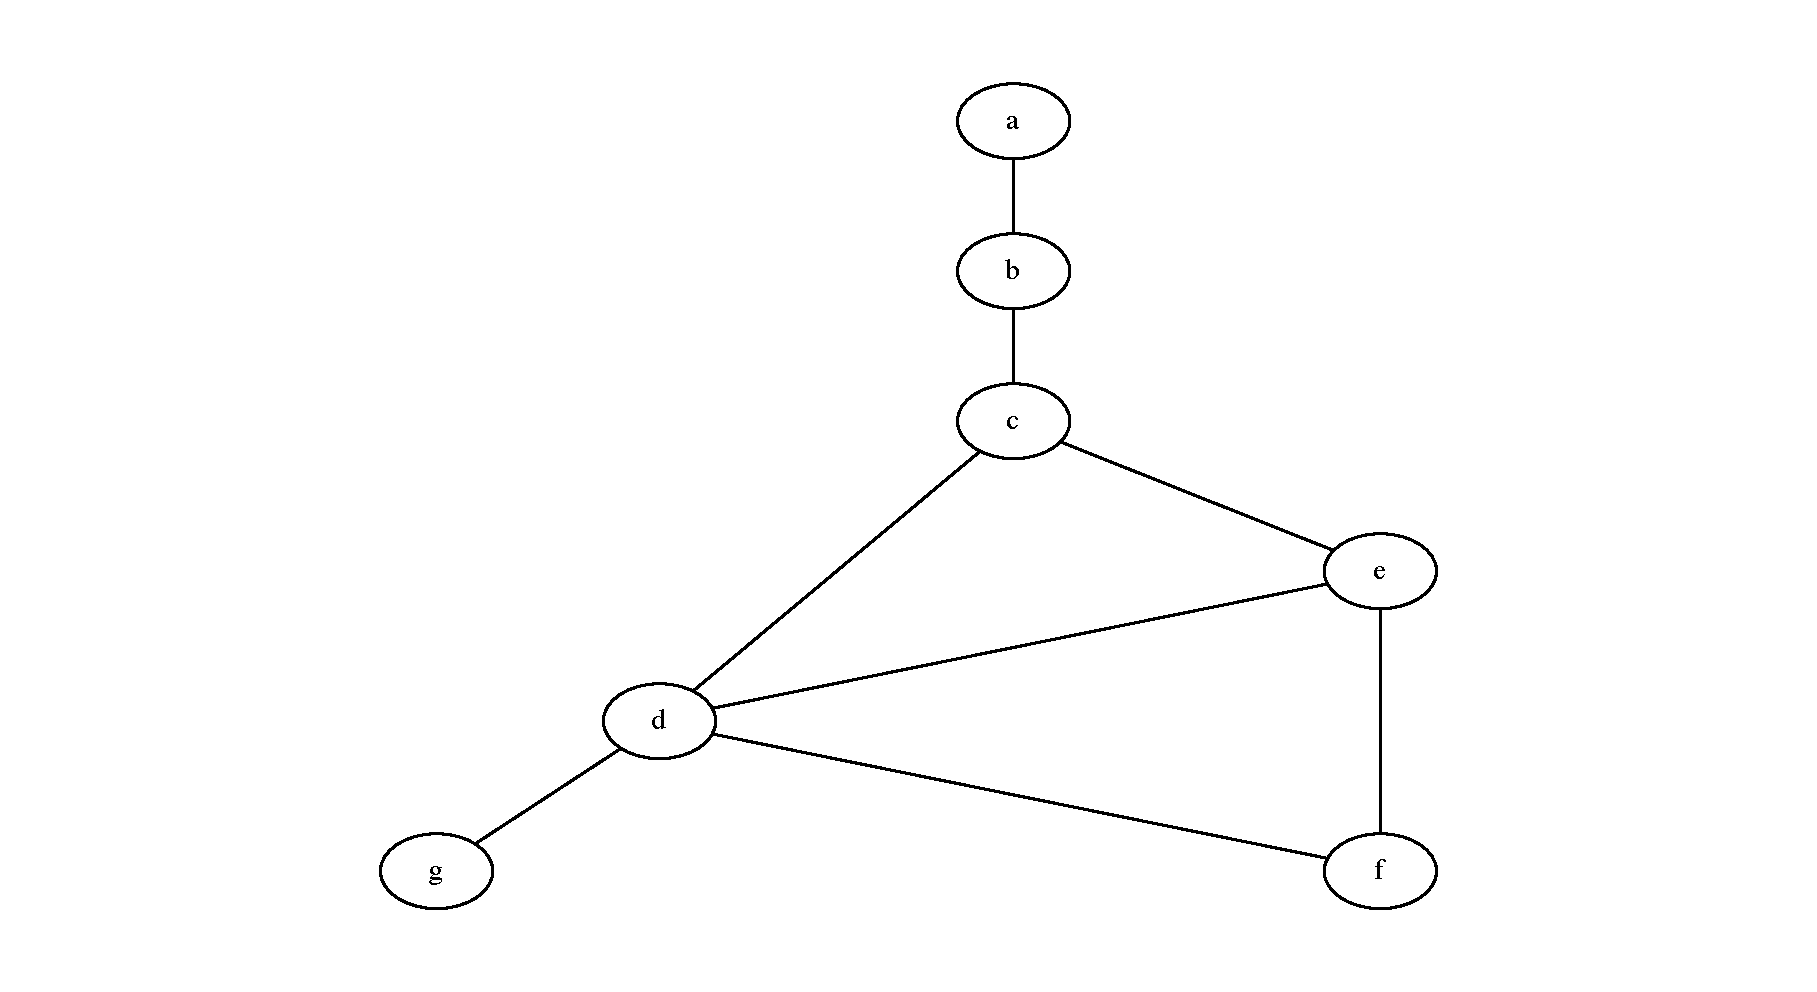
\includegraphics[width=\textwidth]{diagrams/Chapter7_Example1.pdf}
\end{example*}
\begin{algorithm}
\begin{algorithmic}[1]
\State $C \gets \emptyset$
\State $E' \gets E$
\While{$E' \neq \emptyset$}
	\State Choose an edge $\{u,v\}$ in $E'$.
	\State $C \gets C \cup \{u,v\}$
	\State Remove all edges from $E'$ with the end point $u$ or $v$.
\EndWhile
\end{algorithmic}
\caption{APPROX-VERTEX-COVER($G=(V,E)$)}
\end{algorithm}




















\begin{lemma}
If the order in which the candidates appear is random then the average cost of finding a suitable employee is
$ O( c_E *  \ln n + C_I * n)$
\end{lemma}

\textbf{Question:}
How can we know that the order is random ?\\

\subsection{Randomized Algorithms}
In order to guarantee randomness of the input, we randomize it. 

\begin{example}{Hiring}
Given the list of the n candidates, use random numbers to select a candidate for an interview.
$RANDOM(a,b)$ produces an integer z with  $a \leq z \leq b$ where all numbers in this interval are equally probable. 
$RANDOM(0,1)$ produces 0 or 1 with equal probability $\frac{1}{2}$
$RANDOM(3,7)$ produces 4 with probability $\frac{1}{5}$ \\

\textbf{Randomized-Assistant Search}
\begin{enumerate}[label={\arabic*.}]
 \item Permute the list of candidates using a  random number generator
 \item best = 0
 \item ... as before
\end{enumerate}

\begin{lemma}
The expected cost for hiring using the randomized assistant search algorithm is \\
$O( c_E * \ln n + C_I * n)$
\end{lemma}
How to randomize an in input of n elements [A[1...n]]? \\
PERMUTE–BY–SORTING(A) \\
1.	n = length(A) \\
2.	for i = 1...n do \\
3.	P[i] = RANDOM [1, $n^3$] (something arbitrary bigger than n) \\
4.	Sort the array A using P as sort keys \\
5.	return A \\
\newline
RANDOMIZE–IN–PLACE(A) \\
1.	n = length (A) \\
2.	for i= 1 …. n do \\
3.	  swap A[i] $\Leftrightarrow$  A[RANDOM(i,n)] \\

